
\section{Operads and props} \label{s:operads and props}

We consider the category $\Ch$ of differential graded $R$-modules as our base category, remarking that all definitions in this section apply to general closed symmetric monoidal categories.

\subsection{$\S$-modules and $\S$-bimodules} \label{ss:symmetric (bi)modules}

Recall that a group $G$ can be thought of as a category with a single object and only invertible morphisms. From this viewpoint, a left $G$-module (resp. right $G$-module or $G$-bimodule) is the same as a functor from $G$ (resp. $G^\op$ or $G \times G^\op$) to $\Ch$.

Let $\S$ be the category whose objects are the natural numbers and whose set of morphisms between $m$ and $n$ is empty if $m \neq n$ and is otherwise the symmetric group $\S_n$.
A \textit{left $\S$-module} (resp. right $\S$-module or $\S$-bimodule) is a covariant functor from $\S$ (resp. $\S^\op$ or $\S \times \S^\op$) to $\Ch$.
In this paper we prioritize left module structures over their right counterparts. As usual, taking inverses makes both perspectives equivalent.

The homomorphisms $\S_n \to \S_n \times \S_1$ and $\S_n^\op \to \S_1 \times \S_n^\op$ induce natural forgetful functors $\Uleft$ and $\Uright$ from the category of $\S$-bimodules to those of left and right $\S$-modules.

Given a chain complex $C$ define:
\begin{align*}
\End^C(r) &= \Hom(C, C^{\otimes r})
& \End_C(r) &= \Hom(C^{\otimes r}, C)
&\End^C_C(r, s) &= \Hom(C^{\otimes r}, C^{\otimes s})
\end{align*}
with their natural structures of left $\S$-module, right $\S$-module, and $\S$-bimodule respectively.
The natural forgetful functors from $\S$-bimodules to left and right $\S$-modules send $\End^C_C$ to $\End^C$ and $\End_C$ respectively.

An $\S$-module $M$ for which $M(r)$ is free as a $\Z[\S_r]$-module and whose homology is that of a point is said to be $E_\infty$.

\subsection{Composition structures} \label{ss:composition structure}

Operads an props are $\S$-modules and \mbox{$\S$-bimodules} respectively enriched with certain composition structures. These are best understood by abstracting the composition structure naturally present in the $\S$-module $\End^C$, naturally an operad, and the $\S$-bimodule $\End^C_C$, naturally a prop.

Succinctly, an operad $\mathcal O$ is an $\S$-module together with a collection of $R$-linear maps
\begin{equation*}
\mathcal O(r) \otimes \mathcal O(s) \to \mathcal O(r+s-1)
\end{equation*}
satisfying suitable associativity, equivariance and unitality conditions.
A prop $\mathcal P$ is an $\S$-bimodule together with two types of compositions; horizontal
\begin{equation*}
\mathcal P(r_1, s_1) \otimes \mathcal P(r_2, s_2) \to \mathcal P(r_1 + r_2, s_1 + s_2)
\end{equation*}
and vertical
\begin{equation*}
\mathcal P(r,s) \otimes \mathcal P(s, t) \to \mathcal P(r, t)
\end{equation*}
satisfying their own versions of associativity, equivariance and unitality.
For a complete presentation of these concepts we refer to Definition 11 and 54 of \cite{Markl08}.

The compositional structure of a prop $\mathcal P$ restricts to operad structures on $\Uleft(\mathcal P)$ and $\Uright(\mathcal P)$.

An $E_\infty$-operad is an operad whose underlying $\S$-modules is $E_\infty$.

\subsection{Representations} \label{ss:representations}

A morphisms of operads or of props is simply a morphisms of their underlying $\S$-modules or $\S$-bimodules preserving the respective compositional structures.

Consider a chain complex $C$, an operad $\mathcal O$ and a prop $\mathcal P$. An $\mathcal O$-\textit{coalgebra} (resp. $\mathcal O$-\textit{algebra}) structure on $C$ is an operad morphism $\mathcal O \to \End^C$ (resp. $\mathcal O \to \End_C$), and a $\mathcal P$-\textit{bialgebra} structure on $C$ is a prop morphism $\mathcal P \to \End_C^C$.

We remark that the linear duality functor naturally transforms an $\mathcal O$-coalgebra structure on a chain complex into an $\mathcal O$-algebra structure on its dual.

\subsection{Free operads and props} \label{ss:free props}

As described for example in \cite{Markl08}, the \textbf{free prop} $F(M)$ generated by a \mbox{$\S$-bimodule} $M$ is constructed using open directed graphs with no directed loops that are enriched with a labeling described next. We think of each directed edge as built from two compatibly directed half-edges. For each vertex $v$ of a directed graph $G$, we have the sets $in(v)$ and $out(v)$ of half-edges that are respectively incoming to and outgoing from $v$. Half-edges that do not belong to $in(v)$ or $out(v)$ for any $v$ are divided into the disjoint sets $in(G)$ and $out(G)$ of incoming and outgoing external half-edges. For any positive integer $n$, let $\overline{n} = \{1,\dots,n\}$ and $\overline{0} = \emptyset$. For any finite set $S$, denote the cardinality of $S$ by $|S|$. The labeling is given by bijections  
\begin{equation*}
\overline{|in(G)|}\to in(G), \qquad
\overline{|out(G)|}\to out(G),
\end{equation*}
and
\begin{equation*}
\overline{|in(v)|}\to in(v), \qquad
\overline{|out(v)|}\to out(v),
\end{equation*}
for every vertex $v$.
We refer to the isomorphism classes of such labeled directed graphs with no directed loops as $(n,m)$\textbf{-graphs} denoting the set of these by $\G(m,n)$.
We use graphs immersed in the plane to represent elements in $\G(m,n)$, please see Figure \ref{f:immersion}.
We consider the right action of $\S_n$ and the left action of $\S_m$ on a $(n,m)$-graph given respectively by permuting the labels of $in(G)$ and $out(G)$. This action defines the $\S$-bimodule structure on the free prop
\begin{equation} \label{e:free prop}
F(M)(m,n) \ = \bigoplus_{\Gamma \in \G(m,n)} \bigotimes_{v \in Vert(\Gamma)} out(v) \otimes_{\S_q} M(p, q) \otimes_{\S_p} in(v),
\end{equation}
where we simplified the notation writing $p$ and $q$ for $\overline{|in(v)|}$ and $\overline{|out(v)|}$ respectively. The composition structure is defined by (relabeled) grafting and union.

\begin{tikzpicture}[scale=.6]
\draw (1,3.7) to (1,3); 

\draw (1,3) to [out=205, in=90] (0,0);

\draw [shorten >= 0cm] (.6,2.73) to [out=-100, in=90] (2,0);

\draw [shorten >= .15cm] (1,3) to [out=-25, in=30, distance=1.1cm] (1,1.5);
\draw [shorten <= .1cm] (1,1.5) to [out=210, in=20] (0,1);

\node at (1,3.9){};
\node at (0,-.32){};
\node at (2,-.32){};

\node at (3,1.5){$\sim$\ \ \ };
\end{tikzpicture}
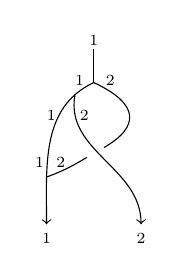
\begin{tikzpicture}[scale=.6]
\draw (1,3.7) to (1,3); 

\draw [->](1,3) to [out=205, in=90] (0,0);

\draw [shorten >= 0cm,->] (.6,2.73) to [out=-100, in=90] (2,0);

\draw [shorten >= .15cm] (1,3) to [out=-25, in=30, distance=1.1cm] (1,1.5);
\draw [shorten <= .1cm] (1,1.5) to [out=210, in=20] (0,1);


\def\x{.8}

\node[scale=\x] at (1,3.9){$\scriptstyle 1$};

\node[scale=\x] at (.7,3.05){$\scriptstyle 1$};
\node[scale=\x] at (1.35,3.05){$\scriptstyle 2$};

\node[scale=\x] at (.1,2.3){$\scriptstyle 1$};
\node[scale=\x] at (.8,2.3){$\scriptstyle 2$};

\node[scale=\x] at (-.15,1.3){$\scriptstyle 1$};
\node[scale=\x] at (.3,1.3){$\scriptstyle 2$};

\node[scale=\x] at (0,-.3){$\scriptstyle 1$};
\node[scale=\x] at (2,-.3){$\scriptstyle 2$};
\end{tikzpicture}

We remark that the free operad construction is described analogously using either graphs with a single input or output and only grafting.

\subsection{The prop $\M$} \label{ss:the prop M}

Let us consider the free prop $F(N)$ generated by the $\S$-bimodule $N$ whose only non-zero chain complexes are concentrated in degree $0$ and are give by
\begin{equation*}
N(1, 0)_0 = \Z\{\varepsilon\}, \qquad
N(1, 2)_0 = \Z[\S_2]\{\Delta\}.
\end{equation*}
Define $\A$ as the quotient of $F(N)$ by the prop ideal generated by the relations
\begin{equation*}
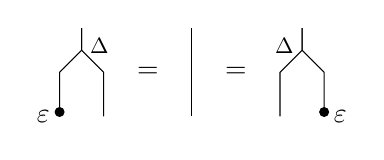
\begin{tikzpicture}[scale=.28]
\draw (-4,0)--(-4,2)--(-5,3)--(-5,4);
\draw (-6,0)--(-6,2)--(-5,3)--(-5,4);
\node [scale=.8] at (-4.2,3.2) {$\Delta$};
\draw [fill] (-6,.2) circle [radius=.2];
\node [left] at (-6,0) {$\varepsilon$};

\node at (-2,2) {=};
\draw (0,0)--(0,4);
\node at (2,2) {=};

\draw (4,0)--(4,2)--(5,3)--(5,4);
\draw (6,0)--(6,2)--(5,3)--(5,4);
\node [scale=.8] at (4.2,3.2) {$\Delta$};
\draw [fill] (6,.2) circle [radius=.2];
\node [right] at (6,0) {$\varepsilon$};
\end{tikzpicture}
\qquad \qquad
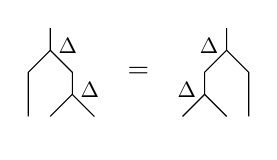
\begin{tikzpicture}[scale=.28]
\node at (0,2){=};
\node at (0,0) {\phantom{$\varepsilon$}};

\draw (2,0)--(3,1)--(3,2)--(4,3)--(4,4);
\draw (4,0)--(3,1);
\draw (4,3)--(5,2)--(5,0);
\node [scale=.8] at (3.2,3.2) {$\Delta$};
\node [scale=.8] at (2.2,1.2) {$\Delta$};

\draw (-2,0)--(-3,1)--(-3,2)--(-4,3)--(-4,4);
\draw (-4,0)--(-3,1);
\draw (-4,3)--(-5,2)--(-5,0);
\node [scale=.8] at (-3.2,3.2) {$\Delta$};
\node [scale=.8] at (-2.2,1.2) {$\Delta$};
\end{tikzpicture}
\end{equation*}
We remark that representations of the prop $\A$ correspond to coassociative counital coalgebra.

Let $W^{(1)}$ be the chain complex of free $\Z[\S_2]$-modules
\begin{equation*}
\begin{tikzcd}
\Z[\S_2]\{\nu\} &[0pt] \arrow[l, "1-T"'] \Z[\S_2]\{\mu\},
\end{tikzcd} 
\end{equation*}
which is isomorphic to the cellular chains on the standard model of the circle
\begin{equation*}
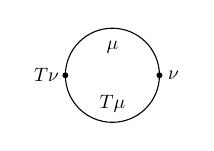
\begin{tikzpicture}[scale=.85]
\draw (0,0) circle (20pt);
\node[scale=.7] at (0,12pt){$\mu$};
\node[scale=.7] at (0,-12pt){$T \mu$};
\node[scale=.7] at (-28pt,0){$T \nu$};
\node[scale=.7] at (26pt,0){$\nu$};
\draw [fill] (-20pt,0) circle [radius=1pt];
\draw [fill] (20pt,0) circle [radius=1pt];
\end{tikzpicture}
\end{equation*}
and let $W^{(0)}$ be the subcomplex generated by $\nu$. We think of $W^{(1)}$ as an $\S_2$-equivariant 1-cell with boundary $W^{(0)}$.

We regard these complexes as $\S$-bimodules concentrated in biarity $(2,1)$, and let $\varphi \colon W^{(0)} \to \A$ be define by sending $T \nu$ and $\nu$ respectively to
\begin{equation*}
	\begin{tikzpicture}[scale=.2]
	\draw (-4,0)--(-4,4);
	\draw (-6,0)--(-6,4);
	\draw [fill] (-6,.2) circle [radius=.2];
	\node [left] at (-6,0) {$\varepsilon$};
	
	\node at (0,.4) {and};
	
	\draw (4,0)--(4,4);
	\draw (6,0)--(6,4);
	\draw [fill] (6,.2) circle [radius=.2];
	\node [right] at (6,0) {$\varepsilon$.};
	\end{tikzpicture}
\end{equation*}
Consider the push-out
\begin{equation*}
\begin{tikzcd}
F(W^{(0)}) \arrow[r, "F(\varphi)"] \arrow[d] & \A \arrow[d, dashed] \\
F(W^{(1)}) \arrow[r, dashed] & \mu \vee \A
\end{tikzcd}
\end{equation*}
in the category of props. We think of $\mathcal A \vee_\varphi \mu$ as the prop obtained by attaching a $1$-cell in biarity $(2,1)$ to $\A$.

Define $\M$ as the quotient of $\mu \vee \A$ by the ideal generated by
\begin{equation*}
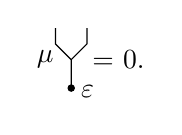
\begin{tikzpicture}[scale=.2]
\draw (5,4)--(5,3)--(6,2)--(6,0);
\draw (7,4)--(7,3)--(6,2);
\node [left] at (5.5,2) {$\mu$};
\draw [fill] (6,.2) circle [radius=.2];
\node [right] at (6,0) {$\varepsilon$};

\node at (9,2) {= 0.};
\end{tikzpicture}
\end{equation*}

We can give a more explicit description of $\M$ using the constructions of Subsection~\ref{ss:free props}.
Consider the $(m,n)$-graphs which we identify with $\varepsilon$, $\Delta$, and $\mu$:
\begin{equation*}
\counit \in \mathcal M(1,0)_0, \hspace*{.6cm} \coproduct \in \mathcal M(1,2)_0, \hspace*{.6cm} \product \in \mathcal M(2,1)_1.
\end{equation*}
Any element in $\M(m,n)$ can be written as a linear combination of the $(m,n)$-graphs generated by these three by grafting, disjoint union and relabeling, modulo the ideals generated by the relations
\begin{equation*}
\qquad \leftcounitality \, , \qquad \rightcounitality \, , \qquad \coassociativity \, , \qquad \productcounit \, .
\end{equation*}
Its chain complex structure is determined using \eqref{e:free prop} by 
\begin{equation*}
\partial\ \counit = 0, \hspace*{.6cm} \partial \ \coproduct = 0, \hspace*{.6cm} \partial \ \product = \ \boundary \, .
\end{equation*}

\begin{proposition}[\cite{Medina20prop1}]
	The operad $\Uleft(\M)$ is an $E_\infty$-operad.
\end{proposition}

We remark that the coassociativity relation is not needed for this result to hold.
We have added it since the counital coalgebras we consider in this work, the Alexander-Whitney coalgebra and the Serre coalgebra are coassociative.
In future work, the double loop space we will modeled using the Saneblize-Umble coalgebra which is not coassociative.

\subsection{The Hopf prop structure} \label{ss:hopf prop structure}

We now describe a diagonal map on $\M$, i.e., a chain map $\M(m,n) \to \M(m,n) \otimes \M(m,n)$ for every biarity $(m,n)$ compatible with the prop structure of $\M$.

As can be seen from \eqref{e:free prop}, the $(m,n)$-part of the free prop is defined only up to a choice of total order on the set of vertices of the $(m,n)$-graph involved.
Let $\Gamma \in \G(m,n)$ be a representative of an element in $\M(m,n)$ of degree $d$ and let us choose an order of its vertices.
This order defines a chain map
\begin{equation*}
\begin{tikzcd}[row sep=tiny, column sep=small]
\iota_\Gamma \colon \chains(\square^1)^{\otimes d} \arrow[r] & \M(m,n) \\
\qquad {[0,1]}^{\otimes d} \arrow[r, |->] & \Gamma,
\end{tikzcd}
\end{equation*}
and we define the value of diagonal of $\M$ on $\Gamma$ using the Serre diagonal
\begin{equation} \label{e:diagonal of M}
\Delta(\Gamma) = \iota_\Gamma^{\otimes 2} \circ \Delta \left([0,1]^{\otimes d}\right).
\end{equation}
This definition is independent of the choice of total order on $Vert(\Gamma)$ by Proposition~\ref{p:serre diagonal invariant}, and it is compatible with the relations since

\begin{center}
	\begin{tikzcd}
	\leftcounitcoproduct \arrow[r, "\Delta"] \arrow[d, <->] &[-5pt] \leftcounitcoproduct \otimes \leftcounitcoproduct \arrow[d, <->] \\
	\identity \arrow[r, "\Delta"] & \identity \otimes \identity \, ,
	\end{tikzcd}
	\qquad
	\begin{tikzcd}
	\rightcounitcoproduct \arrow[r, "\Delta"] \arrow[d, <->] &[-5pt] \rightcounitcoproduct \otimes \rightcounitcoproduct \arrow[d, <->] \\
	\identity \arrow[r, "\Delta"] & \identity \otimes \identity \, ,
	\end{tikzcd}
	\qquad
	\begin{tikzcd}
	\productcounit \arrow[r, "\Delta"] \arrow[d, <->] &[-5pt] \counit \, \otimes \productcounit + \productcounit \otimes \, \counit \arrow[d, <->] \\
	0 \arrow[r, "\Delta"] & \, 0.
	\end{tikzcd}
\end{center}
